\documentclass[12pt, titlepage]{article}

\usepackage{fullpage}
\usepackage[round]{natbib}
\usepackage{multirow}
\usepackage{booktabs}
\usepackage{tabularx}
\usepackage{graphicx}
\usepackage{float}
\usepackage{hyperref}
\usepackage{pdfpages}
\usepackage{pdflscape}


\hypersetup{
    colorlinks,
    citecolor=blue,
    filecolor=black,
    linkcolor=red,
    urlcolor=blue
}

\input{../../Comments}
%% Common Parts

\newcommand{\progname}{Measuring Microstructure Changes During Thermal Treatment} % PUT YOUR PROGRAM NAME HERE
\newcommand{\authname}{Team \#30, ReSprint
\\ Edwin Do
\\ Joseph Braun
\\ Timothy Chen
\\ Abdul Nour Seddiki
\\ Tyler Magarelli
} % AUTHOR NAMES                  

\usepackage{hyperref}
    \hypersetup{colorlinks=true, linkcolor=blue, citecolor=blue, filecolor=blue,
                urlcolor=blue, unicode=false}
    \urlstyle{same}
                                


\newcounter{acnum}
\newcommand{\actheacnum}{AC\theacnum}
\newcommand{\acref}[1]{AC\ref{#1}}

\newcounter{ucnum}
\newcommand{\uctheucnum}{UC\theucnum}
\newcommand{\uref}[1]{UC\ref{#1}}

\newcounter{mnum}
\newcommand{\mthemnum}{M\themnum}
\newcommand{\mref}[1]{M\ref{#1}}

\begin{document}

\title{System Design for \progname{}} 
\author{\authname}
\date{\today}

\maketitle

\pagenumbering{roman}

\section{Revision History}

\begin{table}[hp]
\caption{Revision History} \label{TblRevisionHistory}
\begin{tabularx}{\textwidth}{llX}
\toprule
\textbf{Date} & \textbf{Developer(s)} & \textbf{Change}\\
\midrule
Jan 17, 2023 & Abdul Nour & Added Intro, Purpose, and Scope (3,4,5)\\
Jan 17, 2023 & Abdul Nour & Added Project Overview (6)\\
Jan 17, 2023 & Abdul Nour & Added Design of Hardware (9)\\
Jan 18, 2023 & Joseph Braun & Added System Variables (7)\\
Jan 18, 2023 & Joseph Braun & Added Timeline (12)\\
Jan 18, 2023 & Joseph Braun & Added User Interfaces (8)\\
Jan 18, 2023 & Joseph Braun & Added Communication Protocols (11)\\
Jan 18, 2023 & Joseph Braun & Added Reflection answers\\

... & ... & ...\\
\bottomrule
\end{tabularx}
\end{table}

\newpage

\section{Reference Material}

This section records information for easy reference.

\subsection{Abbreviations and Acronyms}

\renewcommand{\arraystretch}{1.2}
\begin{table}[hp]
\caption{Abbreviations and Acronyms} \label{TblAbbreviationsandAcronyms}
\begin{tabular}{|p{2.75cm}|p{14cm}|}
  \toprule		
  \textbf{symbol} & \textbf{description}\\
  \midrule 
  FR & Functional Requirement\\
  NFR & Non-functional Requirement\\
  NFR-L & Non-functional Requirement: Look and Feel Requirement\\
  NFR-U & Non-functional Requirement: Usability and Humanity Requirement\\
  NFR-P & Non-functional Requirement: Performance Requirement\\
  NFR-O & Non-functional Requirement: Operational and Environmental Requirement\\
  NFR-M & Non-functional Requirement: Maintainability and Support Requirement\\
  NFR-S & Non-functional Requirement: Security Requirement\\
  NFR-C & Non-functional Requirement: Cultural Requirement\\
  NFR-H & Non-functional Requirement: Health and Safety Requirement\\
  NFR-I & Non-functional Requirement: Installability Requirement\\
  \progname & Explanation of program name\\
  \wss{...} & \wss{...}\\
  \bottomrule
\end{tabular}
\end{table}

\newpage

\tableofcontents

\newpage

\listoftables

\listoffigures

\newpage

\pagenumbering{arabic}

\section{Introduction}

% [Include references to your other documentation —SS]

\noindent This document outlines the design and implementation plan for ReSprint's system that would be measuring and analyzing data from thermally treated samples. The main risks identified for the project include insufficient data sampling rates from existing measurement hardware and compatibility issues with the outdated operating system on the control computer. To mitigate these risks, the system will aim to be compatible with newer versions of Windows, be able to read and parse data files, perform extensive calculations, and handle real-time data processing. The project will be developed using C\#\ and the Microsoft Visual Studio environment, with ESLint as the linting tool and MochaJS as the unit testing framework as found in the \href{https://github.com/edwin-do/capstoneTeam30/blob/main/docs/VnVPlan/VnVPlan.pdf}{Verification \&\ Validation Plan}. The system boundaries and components found in the \href{https://github.com/edwin-do/capstoneTeam30/docs/HazardAnalysis/HazardAnalysis.pdf}{Hazard Analysis} document include thermally treated samples, a current source, a temperature sensor, a nanovoltmeter, interfaces between the devices and control computer, the control computer, and the software application installed on the control computer. \\

\section{Purpose}

% \wss{Purpose of your design documentation}

% \wss{Point to your other design documents}

\noindent The purpose of the system design document for this project is to provide a detailed and comprehensive plan for the design and implementation of the hardware and electrical components of the project, following the successful completion of the proof of concept demonstration. As outlined in the \href{https://github.com/edwin-do/capstoneTeam30/blob/main/docs/SRS/SRS.pdf}{Software Requirements and Specification} document, this document will add details to the technical requirements and constraints of the system, including any necessary measurements and interfaces as mentioned in the \href{https://github.com/edwin-do/capstoneTeam30/blob/main/docs/HazardAnalysis/HazardAnalysis.pdf}{Hazard Analysis} document. The document will serve as a guide for the development team in terms of the technical aspects of the project, including the necessary hardware and electrical components, and also acts as a reference for stakeholders, including any regulatory bodies, to understand the technical details of the project and ensure compliance with the \href{https://github.com/edwin-do/capstoneTeam30/blob/main/docs/DevelopmentPlan/DevelopmentPlan.pdf}{Development Plan} documentation. This document will be essential for the proper planning, development, and implementation of the hardware and electrical components of the project. \\

\section{Scope}

% \wss{Include a figure that show the System Context (showing the boundary between your system and the environment around it.)}

\noindent The scope of this document includes a comprehensive design plan for the hardware and electrical components of the project. It covers the purpose and scope of the project, an overview of the normal behavior and handling of undesired events, a component diagram, and a connection between requirements and design. The document also includes details on the system variables, including monitored, controlled, and constant variables, as well as the design of the user interfaces. Additionally, the document covers the design of the hardware, electrical components, and communication protocols, with a timeline for the project, and appendices on the interface, hardware, electrical components, communication protocols, and reflection on the project. Overall, the scope of the document is to provide a detailed and technical guide for the development team and a reference for stakeholders to understand the technical aspects of the project and ensure proper planning, development and implementation of the hardware and electrical components of the project. \\

\begin{figure}[H]
\centerline{\includegraphics[scale=0.6]{ScopeDiagram.png}}
\caption{System Context Diagram}
\label{fig}
\end{figure}

\section{Project Overview}

\subsection{Normal Behaviour}

\noindent The normal behavior and operation of the system refers to how the system is expected to function under normal operating conditions. This includes the system's ability to collect, process, and analyze data from thermally treated samples using the existing hardware, such as the nanovoltmeter, current source, and temperature sensor. The system should also be able to communicate with these devices using the appropriate communication protocols and interfaces, and handle any data synchronization issues. Additionally, the system should be able to perform basic calculations on the data and display it in an easy-to-understand format for the user. The system should also be able to handle real-time data processing, allowing for real-time monitoring of the samples. Overall, the normal behavior of the system is to provide accurate and reliable data analysis of thermally treated samples in real-time, allowing the user to make informed decisions based on the data provided. \\

\subsection{Undesired Event Handling}

% \wss{How you will approach undesired events}

\noindent In the event of an unexpected occurrence, the application should quickly transition to a safe state to prevent the acceptance of any invalid data by the system. This will avoid additional errors when the user accesses or alters corrupted or incorrect data. To ensure that all of the measurements expected are retrieved, the system shall make sure to notify the user to double-check the measurement devices and connectivity in case of failure. This approach will ensure that the system remains reliable and provides accurate data to the user. \\

\begin{landscape}
\subsection{Component Diagram}
\begin{figure}[H]
\centerline{\includegraphics[scale=0.5]{ComponentDiagram.png}}
\caption{Component Diagram}
\label{fig}
\end{figure}
\end{landscape}

\subsection{Connection Between Requirements and Design} \label{SecConnection}

% \wss{The intention of this section is to document decisions that are made
%  ``between'' the requirements and the design.  To satisfy some requirements,
%  design decisions need to be made.  Rather than make these decisions implicit,
%  they are explicitly recorded here.  For instance, if a program has security
%  requirements, a specific design decision may be made to satisfy those
%  requirements with a password.}

\begin{table}[H]
	\centering
	\caption{Connection Between Requirements and Design}
	\label{my-label}
	\begin{tabular}{p{0.175\textwidth} p{0.8\textwidth}}
		\hline
		\textbf{\href{https://github.com/edwin-do/capstoneTeam30/blob/main/docs/SRS/SRS.pdf}{Requirements}} & \textbf{Design Decisions} \\ \hline
		FR1 & All software modules except the Remote Access module are used to satisfy this requirement along with the use of all hardware components \\ \hline
		FR2 & Current State, and Output Communication modules contribute to this requirement \\ \hline
		FR3 & Input Communication module and the use of a GPIB serial communication device shall control the sampling rate \\ \hline
		FR4 & In addition to the modules mentioned for FR2, the Graphical Output module would contribute to this requirement \\ \hline
		FR5 & The Remote Access module is responsible for satisfying this requirement \\ \hline
		NFR-L1 & NF-AT1 \\ \hline
		NFR-L2 & NF-AT2 \\ \hline
		NFR-U1 & NF-UT1 \\ \hline
		NFR-U2 & NF-UT2 \\ \hline
		NFR-U3 & NF-UT3 \\ \hline
	    NFR-U4 & NF-UT4 \\ \hline
	    NFR-U5 & NF-UT5\\ \hline
	    NFR-U6 & NF-UT6 \\ \hline
	    NFR-U7 & NF-UT7 \\ \hline
	    NFR-P1 & NF-PT1 \\ \hline
	    NFR-P2 & NF-PT2 \\ \hline
	    NFR-P3 & NF-PT3 \\ \hline
	    NFR-P4 & NF-PT4 \\ \hline
	    NFR-P5 & NF-PT5 \\ \hline
	    NFR-O1 & NF-OT1 \\ \hline
	    NFR-O2 & NF-OT2 \\ \hline
	    NFR-O3 & N/A \\ \hline
	\end{tabular}
\end{table}

\begin{table}[H]
	\centering
	\caption{Connection Between Requirements and Design Continued}
	\label{my-label}
	\begin{tabular}{p{0.175\textwidth} p{0.8\textwidth}}
		\hline
		\textbf{\href{https://github.com/edwin-do/capstoneTeam30/blob/main/docs/SRS/SRS.pdf}{Requirements}} & \textbf{Design Decisions} \\ \hline
         NFR-M1 & N/A \\ \hline
	    NFR-M2 & NF-MT1 \\ \hline
	    NFR-M3 & NF-MT1 \\ \hline
	    NFR-S1 & NF-ST1 \\ \hline
	    NFR-S2 & NF-ST2 \\ \hline
	    NFR-C1 & NF-CT1 \\ \hline
	    NFR-H1 & NF-HT1 \\ \hline
	    NFR-H2 & NF-HT1 \\ \hline
	    NFR-I1 & NF-MT1 \\ \hline
	\end{tabular}
\end{table}

\newpage

\section{System Variables}

%\wss{Include this section for Mechatronics projects}
\noindent Our system contains three main variables: the current being provided from the Current Source, the voltage measured across the sample with the Nano-Voltmeter, and the temperature measured from the sample.

\subsection{Monitored Variables}
	\begin{itemize}
		\item $m$\textunderscore $voltage$: sample voltage
		\item $m$\textunderscore $temp$: sample temperature
	\end{itemize}

\subsection{Controlled Variables}
\begin{itemize}
		\item $c$\textunderscore $current$: current source output
	\end{itemize}

\subsection{Constants Variables}

No constant variables used in this project.

\section{User Interfaces}

%\wss{Design of user interface for software and hardware.  Attach an appendix if
%needed. Drawings, Sketches, Figma}

\noindent A user interface will be designed for the Windows application. Dr. Zurob has provided the team with the previous version of the application, which can be seen in \hyperref[Apx.A]{Appendix A}. We will design our user interface with the same basic layout as the previous version in order to keep the design familar to the user. Updates from the previous design will include changes to the colour scheme, font, and graphics. 

\section{Design of Hardware}

%\wss{Most relevant for mechatronics projects}
%\wss{Show what will be acquired}
%\wss{Show what will be built, with detail on fabrication and materials}
%\wss{Include appendices as appropriate, possibly with sketches, drawings, CAD, etc}

\noindent There are no mechanical hardware components used in this design. 

\section{Design of Electrical Components}

%\wss{Most relevant for mechatronics projects}
%\wss{Show what will be acquired}
%\wss{Show what will be built, with detail on fabrication and materials}
%\wss{Include appendices as appropriate, possibly with sketches, drawings,
%circuit diagrams, etc}

\noindent For this project, we are provided with all of the hardware. Starting with the thermally treated samples, these will be provided by the user and/or Dr. Zurob. The lab is responsible for providing them as they are specific materials that are treated with equipment outside of the scope of our project. The measurement devices along with the current source and the serial communication module are also provided by the lab as the following: 

  \begin{itemize}
    \item Nano-Voltmeter: Keithley 2182A
    \item Multimeter: Hewlett-Packard 3478A
    \item Precision Current Source: Keithley 6220
    \item Serial Communication Module: National Instruments PCI-GPIB IEEE 488.2 Instrument Control Device
  \end{itemize}

\noindent Reference photos of listed components can be found in \hyperref[Apx.C]{Appendix C}. \\

\noindent We are also provided with the control (lab) computer, which has the PCI-GPIB communication card built in. This computer was upgraded with additional RAM memory and an SSD storage by our mechatronics engineers. Further upgrades would be possible, such as the addition of a Wi-Fi card in case the lab does not provide continuous Ethernet connection to the internet. \\

\section{Design of Communication Protocols}

%\wss{If appropriate}
\noindent The hardware will communicate with the application through the PCI-GPIB card. The protocol used by the card is IEEE 488.2. This is an extension of the IEEE 488 protocol, also known as GPIB, which is a short-range digital communications 8-bit parallel multi-master interface bus specification developed by Hewlett-Packard. Some key features of GPIB are:
\begin{itemize}
	\item One bus can support up to 15 devices
	\item Message transactions are hardware handshaked
	\item Data rates may be up to 1 MB/s
\end{itemize}
\noindent The specifications for the particular PCI-GPIB card used in this system (installed on the lab computer) are shown in \hyperref[Apx.D]{Appendix D}. The specifications include information about IEEE 488 compatibility and bus transfer rates.

\section{Timeline}

\begin{figure}[H]
\centerline{\includegraphics[scale=1]{timeline_1.png}}
\end{figure}

\begin{figure}[H]
\centerline{\includegraphics[scale=1]{timeline_2.png}}
\caption{Project Timeline}
\label{fig}
\end{figure}


%\wss{Schedule of tasks and who is responsible}

% \bibliographystyle {plainnat}
% \bibliography{../../../refs/References}

\newpage{}

\appendix

\section{Interface}
\label{Apx.A}

\begin{figure}[H]
\centerline{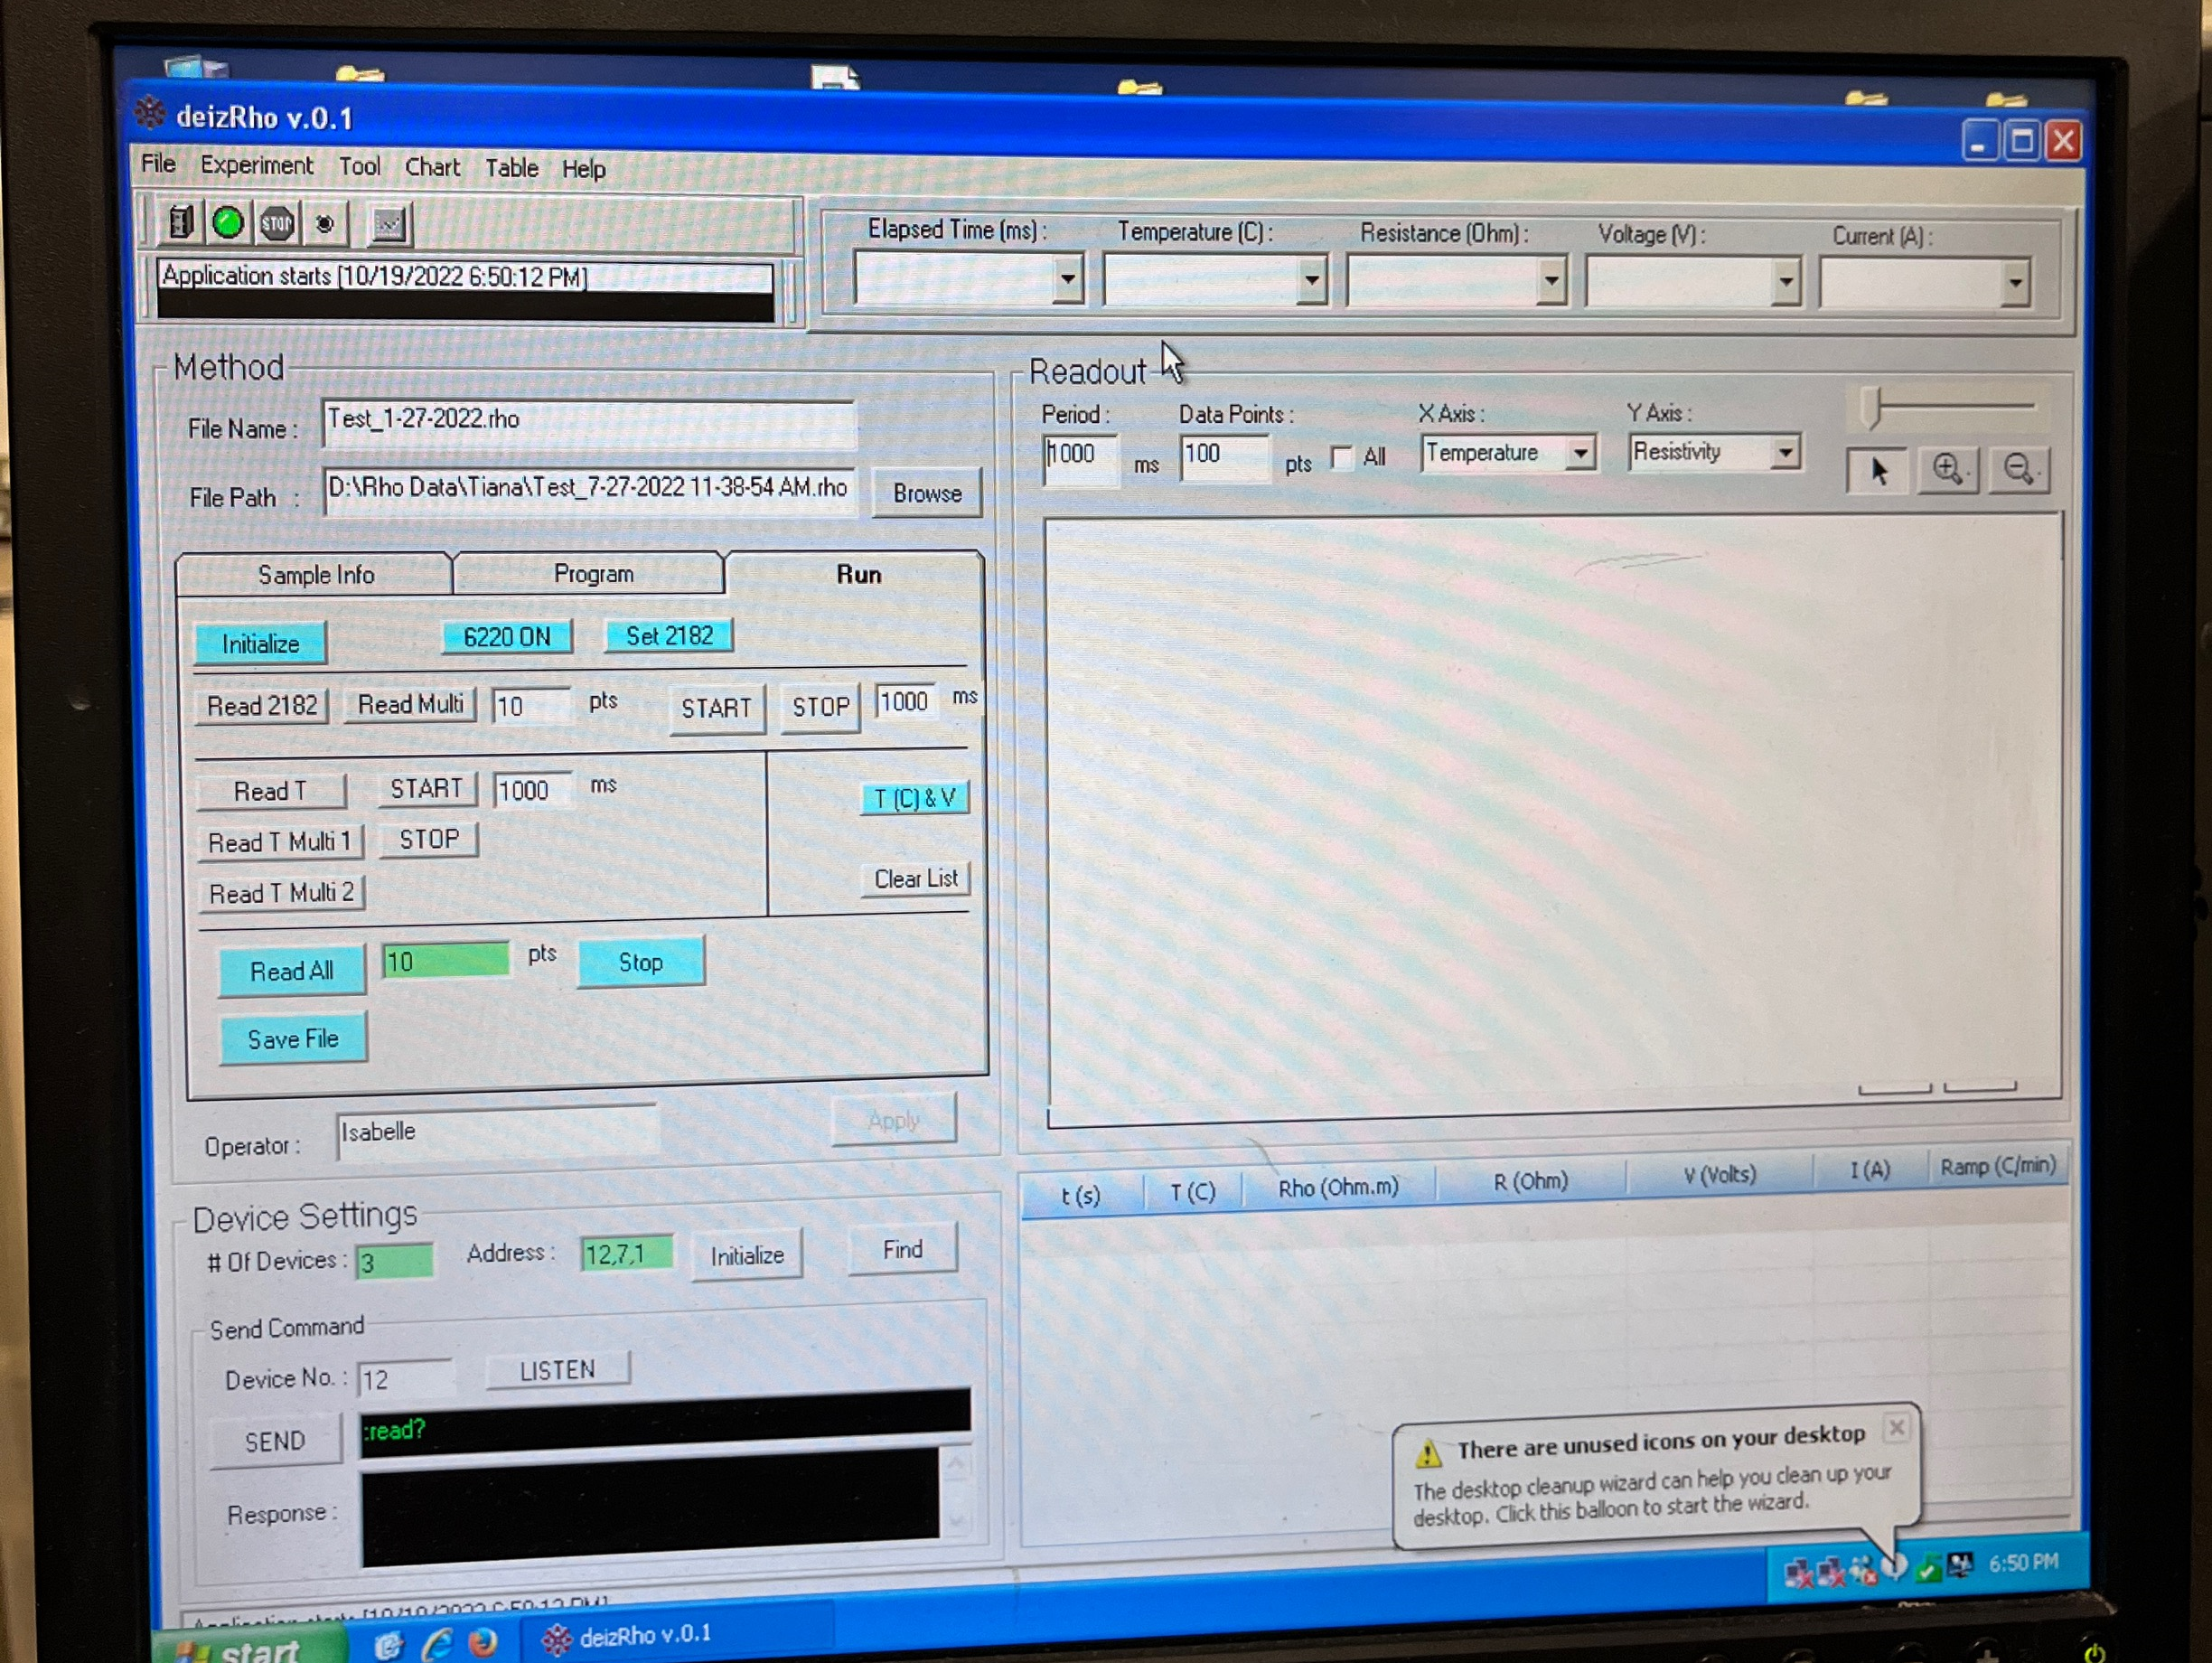
\includegraphics[scale=0.2]{app.png}}
\caption{Previous software user interface design}
\label{fig}
\end{figure}

\section{Mechanical Hardware}
\hfill

\section{Electrical Components}
\label{Apx.C}

\begin{figure}[H]
\centerline{\includegraphics[scale=0.5]{1.jpg}}
\caption{Nano-Voltmeter: Keithley 2182A}
\label{fig}
\end{figure}

\begin{figure}[H]
\centerline{\includegraphics[scale=1]{2.jpg}}
\caption{Multimeter: Hewlett-Packard 3478A}
\label{fig}
\end{figure}

\begin{figure}[H]
\centerline{\includegraphics[scale=0.5]{3.jpg}}
\caption{Precision Current Source: Keithley 6220}
\label{fig}
\end{figure}

\begin{figure}[H]
\centerline{\includegraphics[scale=0.25]{4.png}}
\caption{National Instruments PCI-GPIB IEEE 488.2 Instrument Control Device}
\label{fig}
\end{figure}

\section{Communication Protocols}
\label{Apx.D}

\begin{figure}[H]
\centerline{\includegraphics[scale=1]{specs.png}}
\caption{PCI-GPIB Card Specifications}
\label{fig}
\end{figure}

\section{Reflection}

The information in this section will be used to evaluate the team members on the
graduate attribute of Problem Analysis and Design.  Please answer the following questions:

\begin{enumerate}
  \item What are the limitations of your solution?  Put another way, given
  unlimited resources, what could you do to make the project better? (LO\_ProbSolutions)
  \item Give a brief overview of other design solutions you considered.  What
  are the benefits and tradeoffs of those other designs compared with the chosen
  design?  From all the potential options, why did you select documented design?
  (LO\_Explores)
\end{enumerate}

Answers:
\begin{enumerate}
	\item The main limitations of this project are due to the hardware. We are working with a fairly old desktop computer which was provided for the project. Though we have made some upgrades so that Windows 10 can be run on the computer, we have stopped short of building a new computer. Given unlimited resources, we would purchase all new hardware for the project, including buidling a new computer and replacing all the devices. 
	\item There were primarily two design solutions which our team considered for this project. The first solution was to troubleshoot what went wrong with the old program and fix it so that it could be used again. This solution was proposed due to the low implementation time, as it would be easier to fix the old program than write a new one. The issue with this solution is that ultimately Dr. Zurob is left with the same application he originally had, so there is not much added value. In addition, since the old program runs on Windows XP, there is no possibility of adding a remote connection, which is one of the stretch goals of this project. For these reasons, our team decided to choose our second solution of writing a new program on an updated Windows 10/11 system. The application will have updated graphics and will likely run faster on the updated hardware, and there is the option of adding a remote connection to the application. 
\end{enumerate}


\end{document}